% ****************************************************************************************
% ********************    FUNCIONES, CALCULO DIFERENCIAL, INTEGRAL     *******************
% ****************************************************************************************



% =======================================================
% =======         HEADER FOR DOCUMENT        ============
% =======================================================
    % *********   DOCUMENT ITSELF   **************
    \documentclass[12pt, fleqn]{report}                             %Type of docuemtn and size of font and left eq
    \usepackage[margin=1.2in]{geometry}                             %Margins and Geometry pacakge
    \usepackage{ifthen}                                             %Allow simple programming
    \usepackage{hyperref}                                           %Create MetaData for a PDF and LINKS!
    \hypersetup{pageanchor=false}                                   %Solve 'double page 1' warnings in build
    \setlength{\parindent}{0pt}                                     %Eliminate ugly indentation
    \author{Oscar Andrés Rosas}                                     %Who I am

    % *********   LANGUAJE AND UFT-8   *********
    \usepackage[spanish]{babel}                                     %Please use spanish
    \usepackage[utf8]{inputenc}                                     %Please use spanish - UFT
    \usepackage[T1]{fontenc}                                        %Please use spanish
    \usepackage{textcmds}                                           %Allow us to use quoutes
    \usepackage{changepage}                                         %Allow us to use identate paragraphs

    % *********   MATH AND HIS STYLE  *********
    \usepackage{ntheorem, amsmath, amssymb, amsfonts}               %All fucking math, I want all!
    \usepackage{mathrsfs, mathtools, empheq}                        %All fucking math, I want all!
    \usepackage{centernot}                                          %Allow me to negate a symbol
    \decimalpoint                                                   %Use decimal point

    % *********   GRAPHICS AND IMAGES *********
    \usepackage{graphicx}                                           %Allow to create graphics
    \usepackage{wrapfig}                                            %Allow to create images
    \graphicspath{ {Graphics/} }                                    %Where are the images :D

    % *********   LISTS AND TABLES ***********
    \usepackage{listings}                                           %We will be using code here
    \usepackage[inline]{enumitem}                                   %We will need to enumarate
    \usepackage{tasks}                                              %Horizontal lists
    \usepackage{longtable}                                          %Lets make tables awesome
    \usepackage{booktabs}                                           %Lets make tables awesome
    \usepackage{tabularx}                                           %Lets make tables awesome
    \usepackage{multirow}                                           %Lets make tables awesome
    \usepackage{multicol}                                           %Create multicolumns

    % *********   HEADERS AND FOOTERS ********
    \usepackage{fancyhdr}                                           %Lets make awesome headers/footers
    \pagestyle{fancy}                                               %Lets make awesome headers/footers
    \setlength{\headheight}{16pt}                                   %Top line
    \setlength{\parskip}{0.5em}                                     %Top line
    \renewcommand{\footrulewidth}{0.5pt}                            %Bottom line

    \lhead{                                                         %Left Header
        \hyperlink{chapter.\arabic{chapter}}                        %Make a link to the current chapter
        {\normalsize{\textsc{\nouppercase{\leftmark}}}}             %And fot it put the name
    }

    \rhead{                                                         %Right Header
        \hyperlink{section.\arabic{chapter}.\arabic{section}}       %Make a link to the current chapter
            {\footnotesize{\textsc{\nouppercase{\rightmark}}}}      %And fot it put the name
    }

    \rfoot{\textsc{\small{\hyperref[sec:Index]{Ve al Índice}}}}     %This will always be a footer  

    \fancyfoot[L]{                                                  %Algoritm for a changing footer
        \ifthenelse{\isodd{\value{page}}}                           %IF ODD PAGE:
            {\href{https://compilandoconocimiento.com/yo/}          %DO THIS:
                {\footnotesize                                      %Send the page
                    {\textsc{Oscar Andrés Rosas}}}}                 %Send the page
            {\href{https://compilandoconocimiento.com}              %ELSE DO THIS: 
                {\footnotesize                                      %Send the author
                    {\textsc{Compilando Conocimiento}}}}            %Send the author
    }
    
    
    
% ========================================
% ===========   COMMANDS    ==============
% ========================================

    % =====  GENERAL TEXT  ==========
    \newcommand \Quote {\qq}                                        %Use: \Quote to use quotes
    \newcommand \Over {\overline}                                   %Use: \Bar to use just for short
    \newcommand \ForceNewLine {$\Space$\\}                          %Use it in theorems for example
    
    \newenvironment{Indentation}[1][0.75em]                         %Use: \begin{Inde...}[Num]...\end{Inde...}
    {\begin{adjustwidth}{#1}{}}                                     %If you dont put nothing i will use 0.75 em
    {\end{adjustwidth}}                                             %This indentate a paragraph
    \newenvironment{SmallIndentation}[1][0.75em]                    %Use: The same that we upper one, just 
    {\begin{adjustwidth}{#1}{}\begin{footnotesize}}                 %footnotesize size of letter by default
    {\end{footnotesize}\end{adjustwidth}}                           %that's it


    % =====  GENERAL MATH  ==========
    \DeclareMathOperator \Space {\quad}                             %Use: \Space for a cool mega space
    \DeclareMathOperator \MiniSpace {\;}                            %Use: \Space for a cool mini space
    \newcommand \Such {\MiniSpace|\MiniSpace}                       %Use: \Such like in sets
    \newcommand \Also {\MiniSpace \text{y} \MiniSpace}              %Use: \Also so it's look cool
    \newcommand \Remember[1]{\Space\text{\scriptsize{#1}}}          %Use: \Remember so it's look cool

    \newtheorem{Theorem}{Teorema}[section]                          %Use: \begin{Theorem}[Name]\label{Nombre}...
    \newtheorem{Corollary}{Colorario}[Theorem]                      %Use: \begin{Corollary}[Name]\label{Nombre}...
    \newtheorem{Lemma}[Theorem]{Lemma}                              %Use: \begin{Lemma}[Name]\label{Nombre}...
    \newtheorem{Definition}{Definición}[section]                    %Use: \begin{Definition}[Name]\label{Nombre}...

    \newcommand{\Set}[1]{\left\{ \MiniSpace #1 \MiniSpace \right\}} %Use: \Set {Info}
    \newcommand{\Brackets}[1]{\left[ #1 \right]}                    %Use: \Brackets {Info} 
    \newcommand{\Wrap}[1]{\left( #1 \right)}                        %Use: \Wrap {Info} 
    \newcommand{\pfrac}[2]{\Wrap{\dfrac{#1}{#2}}}                   %Use: Put fractions in parentesis

    \newenvironment{MultiLineEquation}[1]                           %Use: To create MultiLine equations
        {\begin{equation}\begin{alignedat}{#1}}                     %Use: \begin{Multi..}{Num. de Columnas}
        {\end{alignedat}\end{equation}}                             %And.. that's it!
    \newenvironment{MultiLineEquation*}[1]                          %Use: To create MultiLine equations
        {\begin{equation*}\begin{alignedat}{#1}}                    %Use: \begin{Multi..}{Num. de Columnas}
        {\end{alignedat}\end{equation*}}                            %And.. that's it!


    % =====  LOGIC  ==================
    \DeclareMathOperator \doublearrow {\leftrightarrow}             %Use: \doublearrow for a double arrow
    \newcommand \lequal {\MiniSpace \Leftrightarrow \MiniSpace}     %Use: \lequal for a double arrow
    \newcommand \linfire {\MiniSpace \Rightarrow \MiniSpace}        %Use: \lequal for a double arrow
    \newcommand \longto {\longrightarrow}                           %Use: \longto for a long arrow

    % =====  NUMBER THEORY  ==========
    \DeclareMathOperator \Naturals  {\mathbb{N}}                     %Use: \Naturals por Notation
    \DeclareMathOperator \Primes    {\mathbb{P}}                     %Use: \Naturals por Notation
    \DeclareMathOperator \Integers  {\mathbb{Z}}                     %Use: \Integers por Notation
    \DeclareMathOperator \Racionals {\mathbb{Q}}                     %Use: \Racionals por Notation
    \DeclareMathOperator \Reals     {\mathbb{R}}                     %Use: \Reals por Notation
    \DeclareMathOperator \Complexs  {\mathbb{C}}                     %Use: \Complex por Notation

    % === LINEAL ALGEBRA & VECTORS ===
    \DeclareMathOperator \LinealTransformation {\mathcal{T}}        %Use: \LinealTransformation for a cool T
    \newcommand{\Mag}[1]{\left| #1 \right|}                         %Use: \Mag {Info} 

    \newcommand{\pVector}[1]{                                       %Use: \pVector {Matrix Notation} use parentesis
        \ensuremath{\begin{pmatrix}#1\end{pmatrix}}                 %Example: \pVector{a\\b\\c} or \pVector{a&b&c} 
    }
    \newcommand{\lVector}[1]{                                       %Use: \lVector {Matrix Notation} use a abs 
        \ensuremath{\begin{vmatrix}#1\end{vmatrix}}                 %Example: \lVector{a\\b\\c} or \lVector{a&b&c} 
    }
    \newcommand{\bVector}[1]{                                       %Use: \bVector {Matrix Notation} use a brackets 
        \ensuremath{\begin{bmatrix}#1\end{bmatrix}}                 %Example: \bVector{a\\b\\c} or \bVector{a&b&c} 
    }
    \newcommand{\Vector}[1]{                                        %Use: \Vector {Matrix Notation} no parentesis
        \ensuremath{\begin{matrix}#1\end{matrix}}                   %Example: \Vector{a\\b\\c} or \Vector{a&b&c}
    }

    % MATRIX
    \makeatletter                                                   %Example: \begin{matrix}[cc|c]
    \renewcommand*\env@matrix[1][*\c@MaxMatrixCols c] {             %WTF! IS THIS
        \hskip -\arraycolsep                                        %WTF! IS THIS
        \let\@ifnextchar\new@ifnextchar                             %WTF! IS THIS
        \array{#1}                                                  %WTF! IS THIS
    }                                                               %WTF! IS THIS
    \makeatother                                                    %WTF! IS THIS

    % TRIGONOMETRIC FUNCTIONS
    \newcommand{\Cos}[1]{\cos\Wrap{#1}}                             %Simple wrappers
    \newcommand{\Sin}[1]{\sin\Wrap{#1}}                             %Simple wrappers
    \newcommand{\Tan}[1]{tan\Wrap{#1}}                              %Simple wrappers

    % === COMPLEX ANALYSIS ===
    \newcommand \Cis[1]  {\Cos{#1} + i \Sin{#1}}                    %Use: \Cis for cos(x) + i sin(x)
    \newcommand \pCis[1] {\Wrap{\Cis{#1}}}                          %Use: \pCis for the same ut parantesis
    \newcommand \bCis[1] {\Brackets{\Cis{#1}}}                      %Use: \bCis for the same to Brackets

    % === CALCULUS ===
    \newcommand \MiniDerivate[1][x] {\dfrac{d}{d #1}}               %Use: \MiniDerivate for simple use
    \newcommand \Derivate[2]                                        %Complete Derivate -- [f(x)][x]
        {\dfrac{d \; #1}{d #2}}                                     %Use: \Partial for simple use
    
    \newcommand \MiniUpperDerivate[2]                               %Mini Derivate High Orden Derivate -- [x][1]
        {\dfrac{d^{#2}}{d#1^{#2}}}                                  %Mini Derivate High Orden Derivate
    \newcommand \UpperDerivate[3]                                   %Complete High Orden Derivate -- [f(x)][x][1]
        {\dfrac{d^{#3} \; #1}{d#2^{#3}}}                            %Use: \UpperDerivate for simple use
    
    \newcommand \MiniPartial[1][x] {\dfrac{\partial}{\partial #1}} %Use: \MiniDerivate for simple use
    \newcommand \Partial[2]                                        %Complete Derivate -- [f(x)][x]
        {\dfrac{\partial \; #1}{\partial #2}}                      %Use: \Partial for simple use
    
    \newcommand \MiniUpperPartial[2]                                %Mini Derivate High Orden Derivate -- [x][1] 
        {\dfrac{\partial^{#2}}{\partial #1^{#2}}}                   %Mini Derivate High Orden Derivate
    \newcommand \UpperPartial[3]                                    %Complete High Orden Derivate -- [f(x)][x][1]
        {\dfrac{\partial^{#3} \; #1}{\partial#2^{#3}}}              %Use: \UpperDerivate for simple use


    % =====  GENERAL COLOR  =========
    \definecolor{IndigoMD}{HTML}{3F51B5}                            %Use: Color :D
    \definecolor{DeepPurpleMD}{HTML}{673AB7}                        %Use: Color :D
    \definecolor{TealMD}{HTML}{009688}                              %Use: Color :D        
    \definecolor{BlueGrey800MD}{HTML}{37474F}                       %Use: Color :D
    \definecolor{BlueGrey100MD}{HTML}{CFD8DC}                       %Use: Color :D
    \definecolor{IndigoMD}{HTML}{3F51B5}                            %Use: Color :D
    \definecolor{Green100MD}{HTML}{DCEDC8}                          %Use: Color :D

    \newenvironment{ColorText}[1]{                                  %Use: \begin{ColorText}
        \leavevmode\color{#1}\ignorespaces}                         %That's is!


    % =====  CODE EDITOR =========
    \lstdefinestyle{CompilandoStyle} {                              %This is Code Style
        backgroundcolor=\color{BlueGrey800MD},                      %Background Color  
        basicstyle=\tiny\color{white},                              %Font color
        commentstyle=\color{BlueGrey100MD},                         %Comment color
        stringstyle=\color{TealMD},                                 %String color
        keywordstyle=\color{Green100MD},                            %keywords color
        numberstyle=\tiny\color{TealMD},                            %Size of a number
        frame=shadowbox,                                            %Adds a frame around the code
        breakatwhitespace=true,                                     %Style                       
        breaklines=true,                                            %Style                   
        keepspaces=true,                                            %Style                   
        numbers=left,                                               %Style                   
        numbersep=10pt,                                             %Style 
        xleftmargin=\parindent,                                     %Style 
        tabsize=4                                                   %Style 
    }
 
    \lstset{style=CompilandoStyle}                                  %Use this style


% =====================================================
% ============        COVER PAGE       ================
% =====================================================
\begin{document}
\begin{titlepage}

    \center
    % ============ UNIVERSITY NAME AND DATA =========
    \textbf{\textsc{\Large Proyecto Compilando Conocimiento}}\\[1.0cm] 
    \textsc{\Large Cálculo}\\[1.0cm] 

    % ============ NAME OF THE DOCUMENT  ============
    \rule{\linewidth}{0.5mm} \\[1.0cm]
        { \huge \bfseries Cálculo Diferencial e Integral}\\[1.0cm] 
    \rule{\linewidth}{0.5mm} \\[2.0cm]
    
    % ====== SEMI TITLE ==========
    {\LARGE Funciones, Límites, Derivadas e Integrales}\\[7cm] 
    
    % ============  MY INFORMATION  =================
    \begin{center} \large
    \textbf{\textsc{Autor:}}\\
    Rosas Hernandez Oscar Andres
    \end{center}

    \vfill

\end{titlepage}

% =====================================================
% ========                INDICE              =========
% =====================================================
\tableofcontents{}
\label{sec:Index}
\clearpage



% ////////////////////////////////////////////////////////////////////////////////////////////////////////////////////
% ////////////////////////////////////////   FUNCIONES Y LÍMITES     /////////////////////////////////////////////////
% ////////////////////////////////////////////////////////////////////////////////////////////////////////////////////
\part{Funciones y Límites}

    % ======================================================================================
    % ===========================         FUNCIONES               ==========================
    % ======================================================================================
    \chapter{Funciones}
        \clearpage

        % =====================================================
        % ==========    DEFINICION Y BASES           ==========
        % =====================================================
        \section{Definición}

            % ==================================
            % =========   FORMAL     ===========
            % ==================================
            \subsection*{Definición Formal}
                Usando lo que sabemos de relaciones (tengo un libro de eso :p) podemos recordar
                que las funciones no son mas que una relación entre dos conjuntos $f : A \to B$
                , donde se tiene que cumplir que para cada elemento de $A$ le corresponde un
                solo elemento de $B$.


            % ==================================
            % =========   ALTERNAS   ===========
            % ==================================
            \subsection*{Definiciones Alternas}
            Resulta útil pensar una función como si fuera una máquina.

            Si entra $x$ a la máquina, se acepta como una entrada y la máquina produce una
            salida $f(x)$ de acuerdo con la regla de la función. De este modo, puedes pensar
            el dominio como el conjunto de todas las entradas posibles y el rango como el
            conjunto de todas las salidas posibles.

            % ==================================
            % =====   IDEAS IMPORANTES   =======
            % ==================================
            \subsection{Ideas Importantes}

                Digamos que estamos hablando de una función $f$ cualquiera $f: A \to B$.


                \begin{itemize}
                    \item \textbf{Dominio}:
                        Solemos llamar dominio de $f$ al conjunto $A$.
                        \begin{equation}
                            Dominio = A
                        \end{equation}

                    \item \textbf{Rango}:
                        El rango de la función $f$ es simplemente todos los valores
                        de $f(x)$, o siendo mas exactos matemáticamente es $Rango \subseteq B$
                        donde tenemos que:
                        \begin{equation}
                            Rango = \{ f(x) \Such x \in A \} = f(A)
                        \end{equation}

                    \item \textbf{Variable Independiente}:
                        Llamamos variable independiente a un elemento cualquiera del conjunto $A$.
                        Generalmente usamos el símbolo $x$.

                    \item \textbf{Variable Dependiente}:
                        Llamamos variable independiente a un elemento cualquiera del conjunto $Rango$.
                        Generalmente usamos el símbolo $y$ ó $f(x)$.

                \end{itemize}


                

        % =====================================================
        % ========   CARACTERISTICAS DE FUNCIONES    ==========
        % =====================================================
        \section{Caracteristicas de Funciones}

            



    % ======================================================================================
    % ===========================         LIMITES                 ==========================
    % ======================================================================================
    \chapter{Límites}
        \clearpage

        % =====================================================
        % ==========    DEFINICION Y BASES           ==========
        % =====================================================
        \section{Límites Interesantes}

            % ==================================
            % =========   FORMAL     ===========
            % ==================================
            \subsection{$\lim_{x \to 0} \dfrac{\Sin{x}}{x}$}

                Esta es una de los dos límites más importantes en matemáticas, una de las claves para 
                resolver problemas y sobretodo para construir el concepto de derivadas.


                % ======== DEMOSTRACION ========
                \begin{SmallIndentation}[1em]
                    \textbf{Demostración}:
                    
                    Para esta demostración tendré que volver a hacer dibujitos, porque tengo que
                    probar que para $x \in (0, \frac{\pi}{2})$ tenemos que:

                    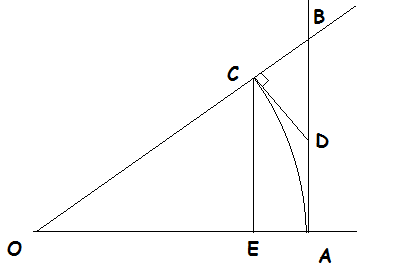
\includegraphics[width=0.40\textwidth]{LimSinx}
                    

                    Sea $x$ el angulo entre $BOA$

                    Primero supongamos que $OC = OA = 1$. Ahora, el camino mas corto de
                    $C$ a $OA$ es $CE$ que es $\Sin{x}$, pero otro camino es la longitud de
                    arco $CA$ que mide $x$ en radianes.

                    Entonces $\Sin{x} < x$.

                    Por otro lado, es obvio que la línea $BA$ es la $tan(x)$ y tenemos que
                    $\Tan{x} = BA = BD+DA > CD+DA > CA = x > \Sin{x}$.

                    Y ahí esta mi clave $\Sin{x} < x < \Tan{x}$.

                    Ahora si multiplicas todo por $\frac{1}{x}$ tenemos que 
                    $\frac{\Sin{x}}{x} < 1 < \frac{\Tan{x}}{x}$, por lo tanto 
                    $\frac{\Sin{x}}{x} < 1$.

                    Y como $1 < \frac{\tan{x}}{x} = \frac{\Sin{x}}{x} \frac{1}{\Cos{x}}$
                    entonces multiplicamos todo por $\Cos{x}$ y tenemos que $\Cos{x} < \Sin{x}{x}$

                    Entonces sabemos que $\Cos{x} < \Sin{x}{x} < 1$, ahora:
                    \begin{itemize}
                        \item $\lim_{x \to 0} \Cos{x} = 1$
                        \item $\lim_{x \to 0} 1 = 1$
                    \end{itemize}

                    Entonces $\Sin{x}{x}$ queda atrapada entre dos funciones que se aproximan a uno
                    cuando $x \to 0$, por lo tanto $\lim_{x \to 0} \dfrac{\Sin{x}}{x} = 1$
                                    
                \end{SmallIndentation}
                    
                


            % ==================================
            % =========   FORMAL     ===========
            % ==================================
            \clearpage
            \subsection{$\lim_{x \to 0} \dfrac{\Cos{x} - 1}{x}$}

                Esta es una de los dos límites más importantes en matemáticas, una de las claves para 
                resolver problemas y sobretodo para construir el concepto de derivadas.

                % ======== DEMOSTRACION ========
                \begin{SmallIndentation}[1em]
                    \textbf{Demostración}:
                    \begin{MultiLineEquation*}{3}
                        \lim_{x \to 0} \dfrac{\Cos{x} - 1}{x}
                            &= \lim_{x \to 0} \pfrac{\Cos{x} - 1}{x} (1)                            
                                && \Remember{Multiplicamos por inocente 1}                         \\
                            &= \lim_{x \to 0} \pfrac{\Cos{x} - 1}{x} \pfrac{\Cos{x}+1}{\Cos{x}+1}   
                                && \Remember{Transformamos el uno}                                  \\
                            &= \lim_{x \to 0} \pfrac{(\Cos{x} - 1)(\Cos{x}+1)}{x(\Cos{x}+1)}     
                                && \Remember{Metemos en la fracción}                                \\
                            &= \lim_{x \to 0} \pfrac{\Cos{x}^2 - 1}{x(\Cos{x}+1)}                   
                                && \Remember{Conjugado}                                             \\
                            &= \lim_{x \to 0} \pfrac{\Sin{x}^2}{x(\Cos{x}+1)}                       
                                && \Remember{$Pitagoras :\Cos{x}^2 -1 = \Sin{x}^2$}                 \\
                            &= \lim_{x \to 0} \pfrac{(\Sin{x}^2)x}{x^2(\Cos{x}+1)}                  
                                && \Remember{Creamos una x arriba y abajo}                          \\
                            &= \lim_{x \to 0} \pfrac{(\Sin{x}^2)}{x^2}\pfrac{x}{\Cos{x}+1}          
                                && \Remember{Separamos}                                             \\
                            &= \lim_{x \to 0} \pfrac{\Sin{x}}{x}^2 \pfrac{x}{\Cos{x}+1}           
                                && \Remember{Vemos que todo esta al cuadrado}                       \\
                            &= \lim_{x \to 0} (1)^2 \pfrac{x}{\Cos{x}+1}                            
                                && \Remember{Recuerda $\lim_{x\to 0} \frac{\Sin{x}}{x} = 0$}        \\
                            &= (1)^2 \pfrac{0}{\Cos{0}+1}                                           
                                && \Remember{Ya no hay indeterminaciones}                           \\
                            &= (1)^2 \pfrac{0}{1+1}                                                 
                                && \Remember{Algebra}                                               \\
                            &= (1)^2 (0)                                                            
                                && \Remember{Todo natural por cero es 0}                            \\
                            &= 0                                                                    
                                && \Remember{Tada! :D}                                              \\
                    \end{MultiLineEquation*}
                        
                
                \end{SmallIndentation}


                % ======== GEOMETRICA ========
                \clearpage
                \begin{SmallIndentation}[1em]
                    \textbf{Interpretación Geométrica}:


                    Este problema es muy importante porque con el podemos demostrar gran cantidad
                    de identidades, pero más que eso, también tiene una muy bonita interpretación
                    geométrica

                    \begin{figure}[h]
                        \centering
                        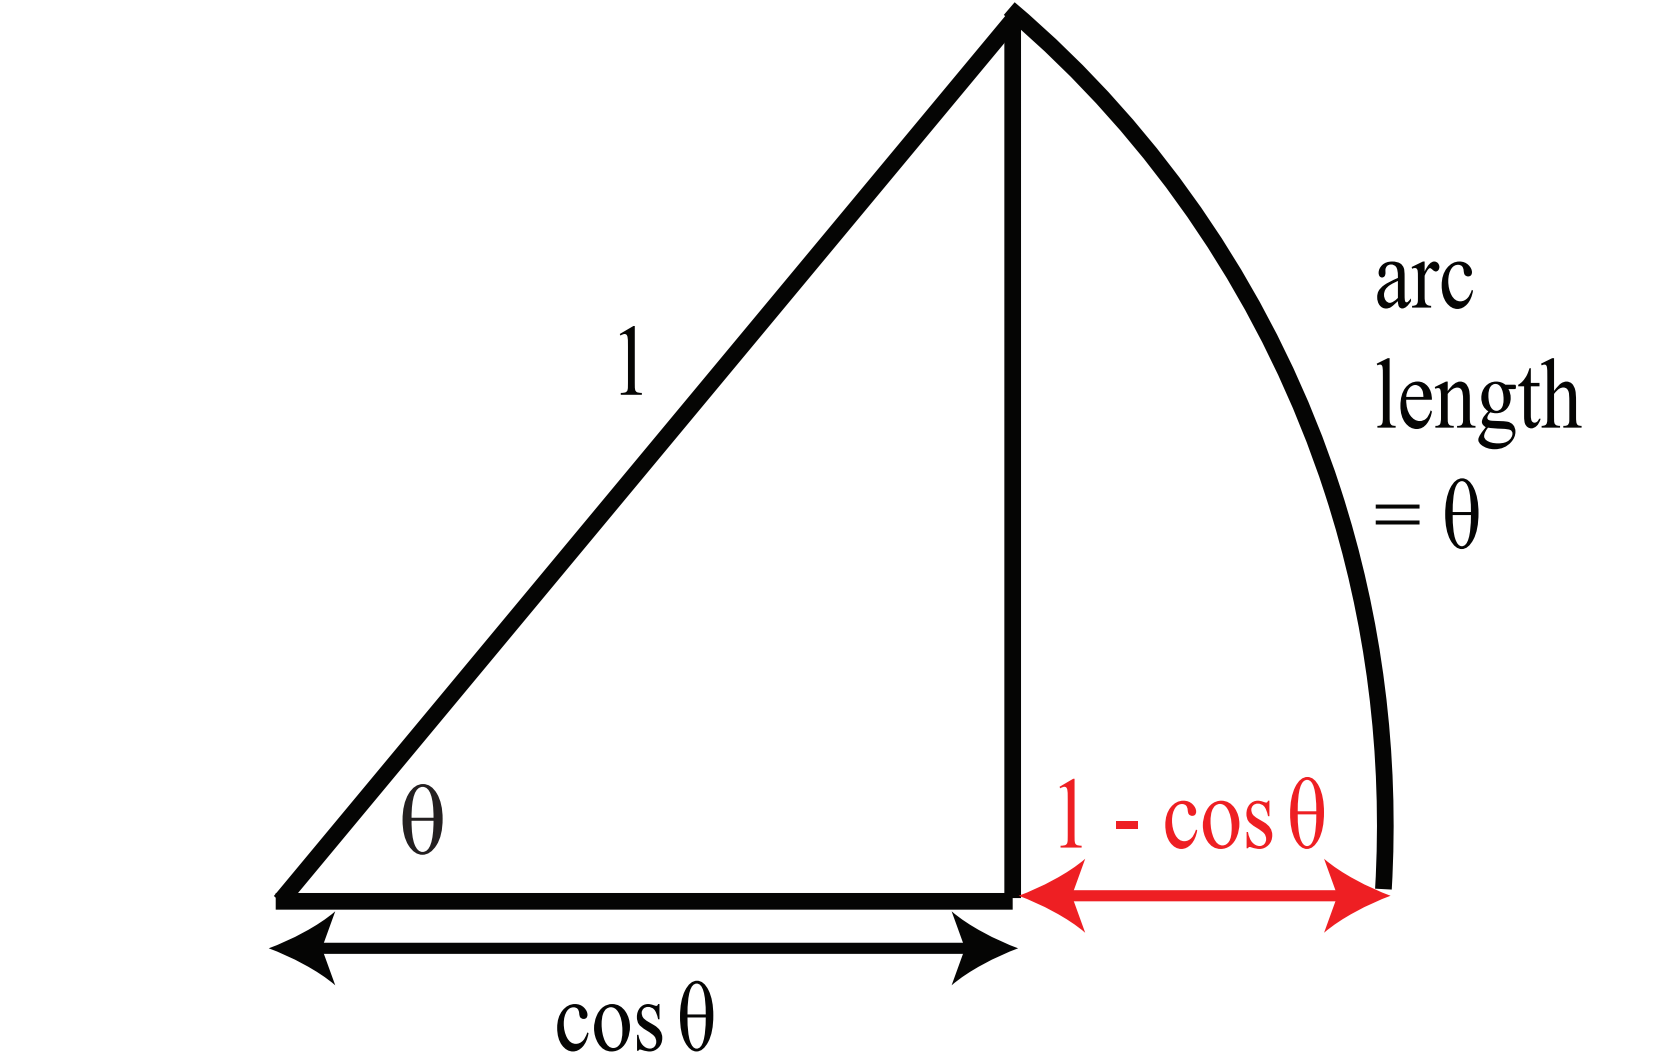
\includegraphics[width=0.45\textwidth]{LimCos-1}
                        \caption{Interpretación geométrica}
                    \end{figure}

                    Para enteder porque nuestro límite da eso, lo que tenemos que ver es
                    que podemos imaginar un circulo de radio uno, de tal manera, que si pusieramos
                    un triangulo rectangulo con un vertice en el origen y el otro tocando a la
                    circunferencia lo que pasaría sería que el otro lado mediría $\Cos{\theta}$

                    Y el espacio que le faltaría a ese vértice para tocar a la circunferencia es
                    $1-\Cos{\theta}$.

                    Lo que en realidad hacemos al momento de tomar el límite cuando $\theta \to 0$
                    es ver que pasa con esa distancia que le falta cuando la longitud de arco
                    de va haciendo más y más pequeña.

                    Y esta claro que mientras más pequeña sea la longitud de arco más pequeño será ese
                    espacio, de hecho podemos hacer que ese espacio se acerqué todo lo que queramos
                    a cero.  
                
                \end{SmallIndentation}
                    
                    











% ////////////////////////////////////////////////////////////////////////////////////////////////////////////////////
% //////////////////////////////////       CALCULO DIFERENCIAL       /////////////////////////////////////////////////
% ////////////////////////////////////////////////////////////////////////////////////////////////////////////////////
\part{Cálculo Diferencial}
















% ////////////////////////////////////////////////////////////////////////////////////////////////////////////////////
% //////////////////////////////////       CALCULO INTEGRAL          /////////////////////////////////////////////////
% ////////////////////////////////////////////////////////////////////////////////////////////////////////////////////
\part{Cálculo Integral}

    % ======================================================================================
    % ========================  INTEGRACION IMPROPIA    ====================================
    % ======================================================================================
    \chapter{Integrales Impropias}
        \clearpage

        % =====================================================
        % ========         INTEGRACION IMPROPIA          ======
        % =====================================================
        \section{Integrales Impropias}

            Al definir la integral definida $\int_a^b f(x) dx$ estamos hablando
            de una función en la que:

            \begin{itemize}
                \item Esta definida en ese intervalo.
                \item No tiene una discontinuidad infinita
                \item Obviamente el intervalo es finito
            \end{itemize}

            Pero, que pasaría si no fuera así...

            Las integrales impropias explorar esta posibilidad así que veasmola:

        % ====================================================
        % ========== INTERVALOS INFINITOS ====================
        % ====================================================
        \clearpage
        \section{Tipo 1: Intervalos Infinitos}

            \subsubsection{Límite Superior}
            Si la $\int_a^t f(x) dx$ existe para todo número $t \geq a$, entonces
            lo siguiente es verdad, siempre que exista el límite (como un número finito).
            \begin{equation}
                \int_a^{\infty} f(x) dx = \lim_{t \to \infty} \int_a^t f(x) dx
            \end{equation}

            \subsubsection{Límite Inferior}
            Si la $\int_t^b f(x) dx$ existe para todo número $b \leq t$, entonces lo
            siguiente es verdad, siempre que exista el límite (como un número finito).
            \begin{equation}
                \int_{- \infty}^b f(x) dx = \lim_{t \to - \infty} \int_t^b f(x) dx
            \end{equation}

            \subsubsection{Convergencia}
            Las integrales impropias $\int_a^{\infty}f(x)dx$ y esta $\int_{-\infty}^bf(x)dx$
            se llaman \textbf{convegentes} si el límite existe y  \textbf{divergente} sino.

            \subsubsection{Ambos Límites}
            Si $\int_a^{\infty}f(x)dx$ y $\int_{-\infty}^bf(x)dx$ son convergentes, entonces
            se define esta asombrosa integral como:
            \begin{equation}
                \int_{-\infty}^{\infty} f(x) dx = \int_{-\infty}^{a} f(x) dx + \int_{a}^{\infty} f(x) dx   
            \end{equation}

            \subsubsection{Ejemplo}
            Podemos ver que con lo que sabemos ya podemos calcular la siguiente integral:

            \begin{equation*}
            \begin{split}
                \int_1^{\infty} \frac{1}{x^2} dx & = \lim_{t \to \infty} \int_1^t \frac{1}{x^2} dx \\
                & = \lim_{t \to \infty} \frac{-1}{x} \big\rvert_{1}^{t} \\
                & = \lim_{t \to \infty} \frac{-1}{t} - \frac{1}{-1} = \frac{-1}{t} + 1 = 1 + \frac{-1}{t} \\
                & = \lim_{t \to \infty} 1 + \frac{-1}{t} = 1 + 0 = 1
            \end{split}
            \end{equation*}

            \clearpage

        % ====================================================
        % ========== INTERVALOS INFINITOS ====================
        % ====================================================
        \clearpage
        \section{Tipo 2: Funciones Discontinuas}

            Si $f(x)$ es continua en $[a, b)$  pero discontinua en b, entonces
            (si el límite existe y es finito):
            \begin{equation}
                \int_a^b f(x) dx = \lim_{t \to b^-} \int_a^t f(x) dx
            \end{equation}

            Si $f(x)$ es continua en $(a, b]$  pero discontinua en a, entonces
            (si el límite existe y es finito):
            \begin{equation}
                \int_a^b f(x) dx = \lim_{t \to a^+} \int_t^b f(x) dx
            \end{equation}



            Si $\int_a^bf(x)dx$ es convergente, entonces se define esta asombrosa integral
            como (donde $c$ es $a<c<b$ ):
            \begin{equation}
                \int_a^b f(x) dx = \int_a^c f(x) dx + \int_c^b f(x) dx  
            \end{equation}




\end{document}